
\documentclass[oneside,a4paper,14pt]{extreport}

% Font tiếng Việt
\usepackage[T5]{fontenc}
\usepackage[utf8]{inputenc}
\DeclareTextSymbolDefault{\DH}{T1}

% Tài liệu tham khảo
\usepackage[
	sorting=nty,
	backend=bibtex,
	defernumbers=true]{biblatex}
\usepackage[unicode]{hyperref} % Bookmark tiếng Việt
\addbibresource{References/references.bib}

\makeatletter
\def\blx@maxline{77}
\makeatother

% Chèn hình, các hình trong luận văn được để trong thư mục Images/
\usepackage{graphicx}
\graphicspath{ {Images/} }
\usepackage{subfig}

% Chèn và định dạng mã nguồn
\usepackage{listings}
\usepackage{color}
\definecolor{codegreen}{rgb}{0,0.6,0}
\definecolor{codegray}{rgb}{0.5,0.5,0.5}
\definecolor{codepurple}{rgb}{0.58,0,0.82}
\definecolor{backcolour}{rgb}{0.95,0.95,0.92}
\lstdefinestyle{mystyle}{
    backgroundcolor=\color{backcolour},   
    commentstyle=\color{codegreen},
    keywordstyle=\color{magenta},
    numberstyle=\tiny\color{codegray},
    stringstyle=\color{codepurple},
    basicstyle=\footnotesize,
    breakatwhitespace=false,         
    breaklines=true,                 
    captionpos=b,                    
    keepspaces=true,                 
    numbers=left,                    
    numbersep=5pt,                  
    showspaces=false,                
    showstringspaces=false,
    showtabs=false,                  
    tabsize=2
}
\lstset{style=mystyle}

% Chèn và định dạng mã giả
\usepackage{amsmath}
\usepackage{algorithm}
\usepackage[noend]{algpseudocode}
\makeatletter
\def\BState{\State\hskip-\ALG@thistlm}
\makeatother

% Bảng biểu
\usepackage{multirow}
\usepackage{array}
\newcolumntype{L}[1]{>{\raggedright\let\newline\\\arraybackslash\hspace{0pt}}m{#1}}
\newcolumntype{C}[1]{>{\centering\let\newline\\\arraybackslash\hspace{0pt}}m{#1}}
\newcolumntype{R}[1]{>{\raggedleft\let\newline\\\arraybackslash\hspace{0pt}}m{#1}}



 
% Đổi tên mặc định
\renewcommand{\chaptername}{Chương}
\renewcommand{\figurename}{Hình}
\renewcommand{\tablename}{Bảng}
\renewcommand{\contentsname}{Mục lục}
\renewcommand{\listfigurename}{Danh sách hình}
\renewcommand{\listtablename}{Danh sách bảng}
\renewcommand{\appendixname}{Phụ lục}

% Định dạng chapter
\usepackage{titlesec}
\titleformat{\chapter}
    [display] 
    {\normalfont\bfseries\Large}{\chaptername \ \thechapter}{10pt}{\huge}
\titlespacing*{\chapter}{0pt}{-10pt}{40pt} %khoảng cách giữa chapter và đầu trang

\titleformat{\section}
    {\normalfont\bfseries\large}{\thesection}{1em}{}
 
\titleformat{\subsection}
    {\normalfont\bfseries\normalsize}{\thesubsection}{1em}{}
  
% Dãn dòng 1.5
\usepackage{setspace}
\onehalfspacing

% Thụt vào đầu dòng
\usepackage{indentfirst}

% Canh lề
\usepackage[
  top=20mm,
  bottom=10mm,
  left=30mm,
  right=20mm,
  footskip = 15mm,
  includefoot]{geometry}
  
% Trang bìa
\usepackage{tikz}
\usetikzlibrary{calc}
\newcommand\HRule{\rule{\textwidth}{1pt}}


\begin{document}

\begin{titlepage}

\begin{center}
%ĐẠI HỌC QUỐC GIA THÀNH PHỐ HỒ CHÍ MINH\\
TRƯỜNG ĐẠI HỌC KHOA HỌC TỰ NHIÊN\\
\textbf{KHOA TOÁN - TIN HỌC}

\begin{figure}[htp]
  \centering
  
\includegraphics[width=8cm]{images/hcmus.png}
  \end{figure}

{\bfseries PYTHON CHO KHOA HỌC DỮ LIỆU\\[1cm] } 



{ \large \bfseriesĐỒ ÁN CUỐI KÌ \\
  \bfseries SUMMARIZING CONSERVATIONS\\[3CM]} 

{\bfseries Giảng viên phụ trách\\}
  Thầy Hà Văn Thảo\\


\begin{tikzpicture}[remember picture, overlay]
  \draw[line width = 2pt] ($(current page.north west) + (2cm,-2cm)$) rectangle ($(current page.south east) + (-1.5cm,2cm)$);
\end{tikzpicture}

\vfill
Tp. Hồ Chí Minh, tháng 12, năm 2024

\end{center}

\end{titlepage}

\pagenumbering{roman} % Đánh số i, ii, iii, ...

% Mục lục
\addcontentsline{toc}{chapter}{Mục lục}
\tableofcontents

\clearpage

\pagenumbering{arabic} % Đánh số 1, 2, 3, ...

% Các chương nội dung

\chapter{Giới thiệu}
\label{Chapter1}

\section{Thông tin nhóm}

\begin{itemize}
    \item 22110215 - Phạm Thị Anh Thư
    \item 22110177 - Phạm Đăng Quang
    \item 22110204 - Nguyễn Thiện Thanh
    \item 22110210 - Võ Xuân Thiện
    \item 22110208 - Nguyễn Ngọc Thiện
\end{itemize}

\section{Mô hình ngôn ngữ lớn}
Ngày 30 tháng 11 năm 2022 đánh dấu một chương quan trọng trong lịch sử của học máy. Đó là ngày OpenAI phát hành ChatGPT, thiết lập một tiêu chuẩn mới cho chatbot được hỗ trợ bởi các Mô hình Ngôn ngữ Lớn và mang đến cho công chúng một trải nghiệm trò chuyện chưa từng có.

Kể từ đó, các mô hình ngôn ngữ lớn - còn được gọi là LLM - đã được công chúng chú ý do số lượng lớn các tác vụ mà chúng có thể thực hiện. Ví dụ bao gồm:
\begin{itemize}

    \item Tóm tắt văn bản: Các mô hình này có thể thực hiện việc tóm tắt các văn bản lớn, bao gồm văn bản pháp lý, đánh giá, hội thoại và nhiều văn bản khác.

    \item Phân tích cảm xúc: Chúng có thể đọc qua các đánh giá về sản phẩm và dịch vụ và phân loại chúng là tích cực, tiêu cực hoặc trung lập. Chúng cũng có thể được sử dụng trong Tài chính để xem liệu công chúng nói chung cảm thấy lạc quan hay bi quan về một số chứng khoán nhất định.

    \item Dịch ngôn ngữ: Chúng có thể cung cấp bản dịch theo thời gian thực từ ngôn ngữ này sang ngôn ngữ khác.

    \item Hệ thống đề xuất dựa trên văn bản: Chúng cũng có thể đề xuất các sản phẩm mới cho khách hàng dựa trên đánh giá của họ về các sản phẩm đã mua trước đó.
\end{itemize}

\section{The Transformer Architecture}
Để hiểu được trạng thái hiện tại của các LLM(mô hình ngôn ngữ lớn), chúng ta phải quay trở lại bài báo "Attention is All You Need" của Google vào năm 2017. Trong bài báo này, kiến trúc Transformer đã được giới thiệu với thế giới, và nó đã thay đổi ngành công nghiệp mãi mãi.

Mặc dù mạng nơ-ron nhân tạo (neural networks) có thể được sử dụng để cho phép máy tính hiểu văn bản, nhưng các mô hình này cực kỳ hạn chế do thực tế là chúng chỉ cho phép máy xử lý từng từ một, dẫn đến việc mô hình không thể nắm bắt được toàn bộ ngữ cảnh của văn bản.

Tuy nhiên, kiến trúc Transformer dựa trên cơ chế chú ý (attention mechanism), cho phép mô hình xử lý toàn bộ câu hoặc đoạn văn cùng một lúc, thay vì từng từ một. Đây là bí mật chính đằng sau khả năng hiểu ngữ cảnh đầy đủ, mang lại sức mạnh lớn hơn cho tất cả các mô hình xử lý ngôn ngữ này.

Việc xử lý đầu vào văn bản với kiến trúc Transformer dựa trên tokenization, là quá trình chuyển đổi văn bản thành các thành phần nhỏ hơn được gọi là token. Đây có thể là từ, từ phụ, ký tự hoặc nhiều thành phần khác.

Các token sau đó được ánh xạ tới các ID số, là duy nhất cho mỗi từ hoặc từ phụ. Mỗi ID sau đó được chuyển đổi thành một embedding: một vectơ dày đặc, nhiều chiều chứa các giá trị số. Các giá trị này được thiết kế để nắm bắt ý nghĩa ban đầu của các token và đóng vai trò là đầu vào cho mô hình Transformer.

Điều quan trọng cần lưu ý là các embedding này có nhiều chiều, với mỗi chiều nắm bắt các khía cạnh nhất định về ý nghĩa của một token. Do bản chất nhiều chiều của chúng, embedding không dễ dàng được con người giải thích, nhưng các mô hình Transformer dễ dàng sử dụng chúng để xác định và nhóm các token có ý nghĩa tương tự trong không gian vectơ.

Bằng cách sử dụng vector này làm đầu vào, mô hình Transformer học cách tạo ra đầu ra dựa trên xác suất của các từ tiếp theo có thể xuất hiện một cách tự nhiên sau một từ đầu vào. Quá trình này được lặp lại cho đến khi mô hình tạo ra toàn bộ đoạn văn bắt đầu từ một câu lệnh ban đầu.

\begin{figure*}[htp]
    \centering
    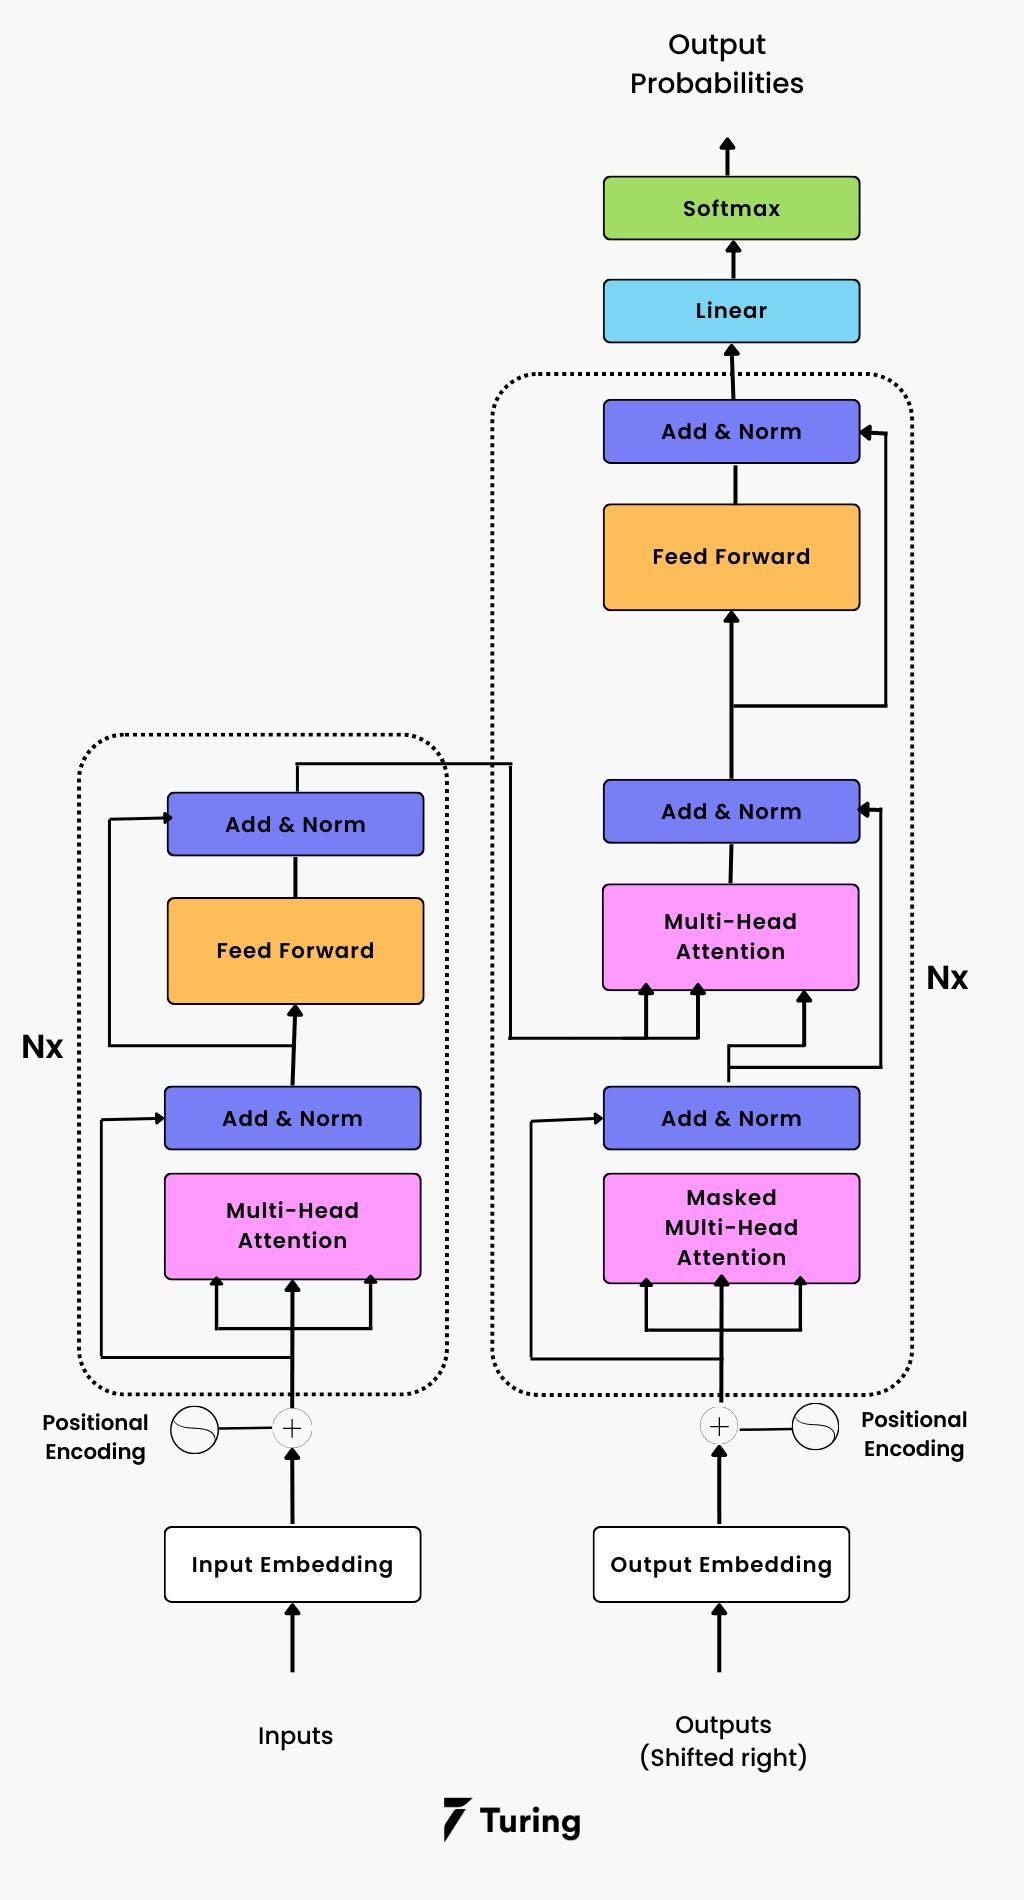
\includegraphics[width=8cm]{images/Transformer_architecture.png}
    \caption{Kiến trúc Transformer}
    \end{figure*}

\section{Mục tiêu}
Mục tiêu của notebook này là để chứng minh cách các Mô hình Ngôn ngữ Lớn (Large Language Models - LLMs) có thể được sử dụng cho một số tác vụ liên quan đến xử lý ngôn ngữ (language processing). Trong trường hợp này, tôi sẽ tận dụng sức mạnh của học chuyển giao (transfer learning) để xây dựng một mô hình có khả năng tóm tắt các cuộc hội thoại (summarizing dialogues).

Nếu các bạn có thể chưa biết, transfer learning là một kỹ thuật học máy (machine learning technique) trong đó chúng ta sử dụng một mô hình được đào tạo trước (pre-trained model) - vốn đã có kiến thức trong một lĩnh vực rộng - và điều chỉnh chuyên môn của nó cho một tác vụ cụ thể (specific task) bằng cách huấn luyện nó trong một tập dữ liệu cụ thể (specific dataset) mà chúng ta có thể có. Quá trình này cũng có thể được gọi là tinh chỉnh (fine-tuning).

Thư viện Transformers - một trong những thư viện phổ biến nhất để làm việc với các tác vụ học sâu (deep learning tasks) - cung cấp khả năng làm việc với các kiến trúc (architectures) sau:\\

\begin{figure*}[htp]
    \centering
    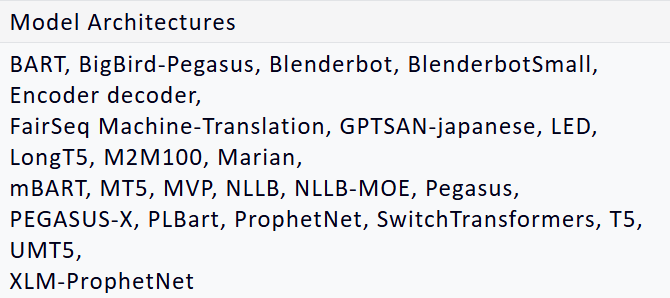
\includegraphics{images/kdl2.png}
    \caption{Các kiến trúc mô hình mà thư viện Transformers hỗ trợ}
    \end{figure*}

Thư viện Transformers cho phép chúng ta dễ dàng tải xuống và tinh chỉnh các mô hình được đào tạo trước tiên tiến, đồng thời cho phép chúng ta dễ dàng làm việc với cả TensorFlow và PyTorch cho một số tác vụ liên quan đến Xử lý Ngôn ngữ Tự nhiên (Natural Language Preprocessing - NLP), Thị giác Máy tính (Computer Vision), Âm thanh (Audio), v.v.


\chapter{Cài đặt}
\label{Chapter2}

\section{Data source}

Theo tài liệu của thư viện Transformers, tóm tắt có thể được mô tả là việc tạo ra một phiên bản ngắn hơn của một tài liệu hoặc một bài báo mà vẫn nắm bắt được tất cả các thông tin quan trọng.

Trong trường hợp này, chúng ta sẽ tóm tắt các cuộc hội thoại bằng cách sử dụng một tập dữ liệu chứa các đoạn chat.

Đối với nhiệm vụ này, chúng ta sẽ sử dụng Tập dữ liệu SamSum, bao gồm ba tệp csv cho huấn luyện, kiểm tra và xác thực. Tất cả các tệp này được cấu trúc thành một id cụ thể, một cuộc hội thoại(a dialogue) và một bản tóm tắt( a summary). Tập dữ liệu SamSum bao gồm các đoạn chat, lý tưởng cho việc tóm tắt các cuộc hội thoại.\\

\lstinputlisting[language=Python]{SourceCode/data.py}

\section{Thư viện}

\lstinputlisting[language=Python]{SourceCode/importlibrary.py}

\section{Chưa rõ}

\lstinputlisting[language=Python]{SourceCode/unknow.py}

\section{Tập dữ liệu}

Chúng ta có thể bắt đầu phân tích tập dữ liệu bằng cách tải tất cả ba tập dữ liệu có sẵn, bao gồm tập huấn luyện (train), tập kiểm tra (test) và tập xác thực (val).\\

\lstinputlisting[language=Python]{SourceCode/explore.py}

\begin{figure*}[htp]
    \centering
    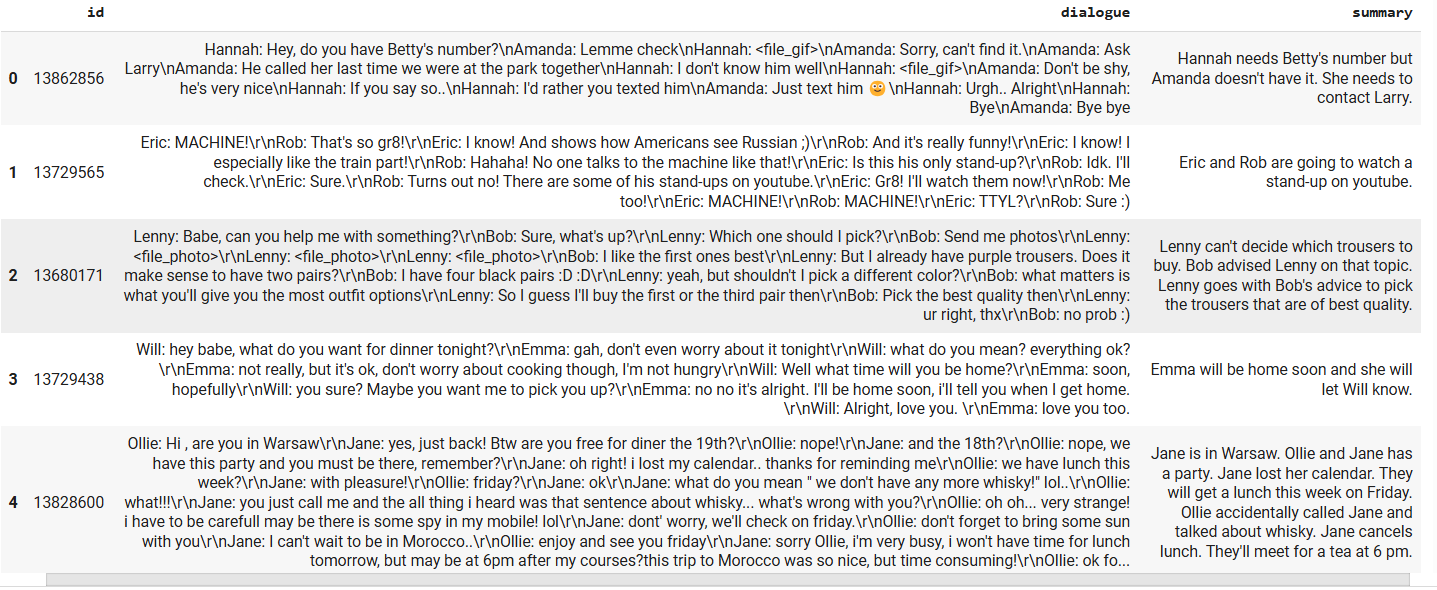
\includegraphics[scale=.5]{images/df.png}
    \caption{Minh họa Dataframe}
    \end{figure*}
\pagebreak



\chapter{Xây dựng mô hình}
\label{Chapter3}
\section{Tiền xử lý dữ liệu}

Chúng ta nhận thấy rằng trong một số đoạn hội thoại sẽ có những thẻ như file photo, hãy xem qua một ví dụ:\\

\begin{figure*}[htp]
    \centering
    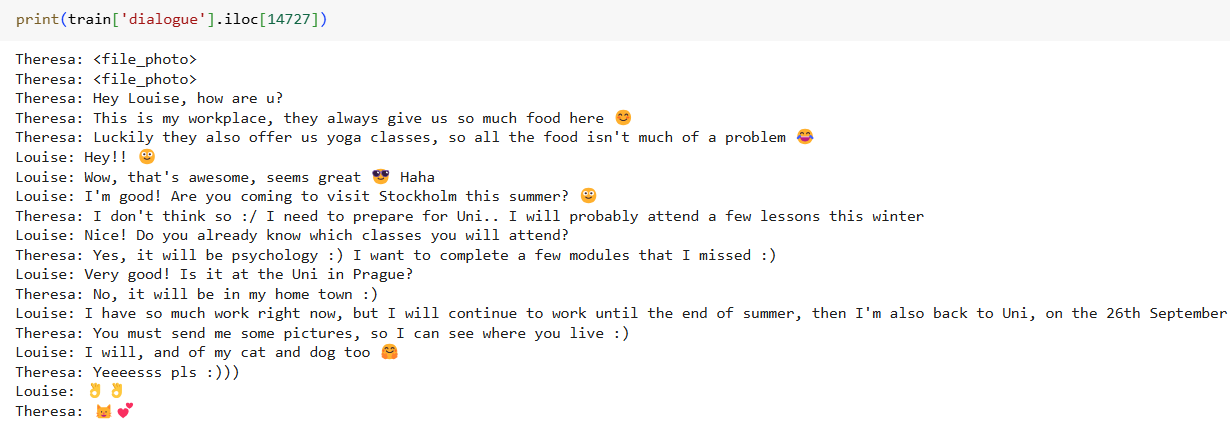
\includegraphics[scale=.6]{images/vd1.png}
    \end{figure*}

Để loại bỏ các thẻ này khỏi văn bản, giúp văn bản trở nên sạch hơn, chúng ta sẽ sử dụng hàm clean-tags được định nghĩa dưới đây:\\

\lstinputlisting[language=Python]{SourceCode/clean_tags.py}


\begin{figure*}[htp]
    \centering
    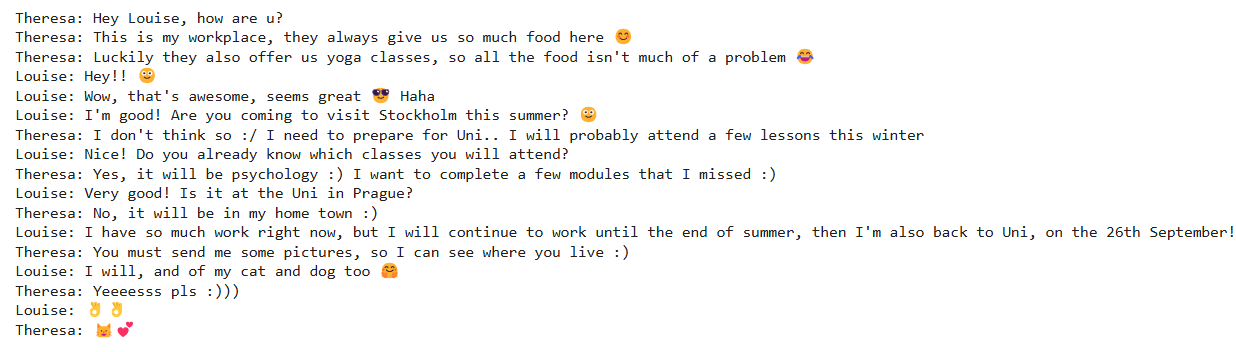
\includegraphics[scale=.6]{images/ketqua.png}
    \end{figure*}

Có thể thấy rằng chúng ta đã loại bỏ thành công các thẻ khỏi văn bản. Bây giờ, chúng ta sẽ định nghĩa hàm clean-df, trong đó sẽ áp dụng hàm clean-tags cho toàn bộ 
các bộ dữ liệu.\\

\lstinputlisting[language=Python]{SourceCode/clean_df.py}

Các thẻ đã được loại bỏ khỏi văn bản. Việc thực hiện quá trình dọn dẹp dữ liệu như vậy là rất có ích để loại bỏ nhiễu - những thông tin không đóng góp đáng kể vào ngữ cảnh tổng thể và có thể làm giảm hiệu suất.

Bây giờ, chúng ta sẽ thực hiện một số bước tiền xử lý cần thiết để chuẩn bị dữ liệu của chúng ta làm đầu vào cho mô hình đã được huấn luyện sẵn và để tinh chỉnh mô hình. Phần lớn những gì chúng ta đang làm ở đây là một phần trong hướng dẫn về Tóm tắt Văn bản được mô tả trong tài liệu của Transformers.

Đầu tiên, chúng ta sẽ sử dụng thư viện Datasets để chuyển các Pandas DataFrame của chúng ta thành Datasets. Điều này sẽ giúp dữ liệu của chúng ta sẵn sàng để xử lý trong toàn bộ hệ sinh thái của Hugging Face.\\

\lstinputlisting[language=Python]{SourceCode/transf.py}

Sau khi chuyển đổi thành công các Pandas DataFrames thành Datasets, chúng ta có thể tiếp tục với quá trình mô hình hóa.\\

\section{Mô hình hóa}
Như chúng ta đã đề cập trước đó, chúng ta sẽ tinh chỉnh một phiên bản của BART đã được huấn luyện trên nhiều bài báo tin tức cho nhiệm vụ tóm tắt văn bản, đó là facebook/bart-large-xsum.
Chúng ta sẽ trình bày ngắn gọn mô hình này bằng cách tải một pipeline tóm tắt với mô hình này để cho bạn thấy cách nó hoạt động trên dữ liệu tin tức.\\

\lstinputlisting[language=Python]{SourceCode/loadbart.py}

Ví dụ, chúng ta sẽ sử dụng bài báo tin tức sau, được xuất bản trên CNN vào ngày 24 tháng 10 năm 2023, với tiêu đề "Bobi, the world's oldest dog ever, died aged 31". Lưu ý rằng đây là một bài báo tin tức hoàn toàn mới mà chúng ta đưa vào mô hình, để có thể xem nó hoạt động như thế nào.\\

\lstinputlisting[language=Python]{SourceCode/new.py}


\begin{figure}[htp]
	\centering
	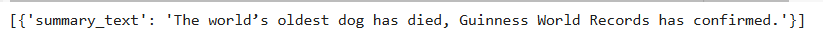
\includegraphics[width=16cm, height=2cm]{images/kq}

\end{figure}

\pagebreak
Bạn có thể quan sát thấy rằng mô hình có thể tạo ra một đoạn văn bản ngắn gọn hơn rất nhiều, chứa đựng thông tin quan trọng nhất từ văn bản đầu vào. Đây là một ví dụ tóm tắt thành công.

Tuy nhiên, mô hình này đã được huấn luyện chủ yếu trên các tập dữ liệu bao gồm nhiều bài báo tin tức từ CNN và Daily Mail, chứ không phải trên nhiều dữ liệu hội thoại. Vì vậy, chúng ta sẽ tiến hành tinh chỉnh nó với SamSum dataset.
    
Bây giờ, chúng ta sẽ tải BartTokenizer và BartForConditionalGeneration sử dụng checkpoint facebook/bart-large-xsum.\\


\include{Chapter4/chapter4}

% In tài liệu tham khảo
\addcontentsline{toc}{chapter}{Tài liệu tham khảo}
\printbibheading[title={Tài liệu tham khảo}]



\end{document} 